% !TeX root = ./main.tex

\chapter*{\large ВВЕДЕНИЕ}
\addcontentsline{toc}{chapter}{ВВЕДЕНИЕ}

Современный этап цифровой трансформации науки, биомедицинской диагностики и инженерного компьютерного моделирования характеризуется переходом от изолированных эмпирических алгоритмов обработки растровых сигналов к физически согласованным информационным технологиям анализа пространственно-временных данных~[\ref{itm:samarsky}, с.~14;~\ref{itm:kharin}, с.~22]. В задачах количественной микроскопии живых клеток, цифровой гистопатологии и экологического мониторинга регистрируемые кадры представляют собой дискретные выборки непрерывного физического поля (интенсивности флуоресценции, концентрации маркера или оптической плотности), эволюционирующего на ограниченной двумерной области.

Ключевая научно-технологическая проблема состоит в том, что пространственное разрешение и топология графа наблюдений существенно различаются между этапом обучения модели и этапом её лабораторной или клинической эксплуатации. При регистрации длительных обучающих серий в цейтраферной флуоресцентной микроскопии операторы применяют аппаратный биннинг пикселей матрицы (усреднение блоков $4\times 4$ или $6\times 6$) для снижения фототоксичности лазерного облучения, подавления фотовыцветания флуорофора и ускорения кадровой развёртки~[\ref{itm:nedzvedz2012}, с.~52]. На этапе же прецизионной морфометрической диагностики обученная модель применяется к кадрам полного разрешения (с ростом числа узлов в $8\text{--}10$~раз), нерегулярным адаптивным триангуляциям Делоне либо графам смежности суперпикселей~[\ref{itm:skimage}].

Классические графовые нейронные сети (ГНС), построенные на комбинаторной передаче сообщений по списку смежности~[\ref{itm:gasnikov}, с.~68;~\ref{itm:grand}], в подобных условиях теряют работоспособность: при измельчении шага сетки $h_G$ разности признаков сжимаются, рёберное внимание искажает масштаб времени, а локальные вентили переключателей вырождаются без переобучения весов~[\ref{itm:a1},~\ref{itm:a3}]. Высокая мировая актуальность проблемы подтверждается более чем $35$-кратным ростом числа научных работ по инвариантным к дискретизации нейронным операторам и графовым уравнениям в частных производных (УЧП) в архиве \texttt{arXiv.org}~[\ref{itm:arxiv}] и в базе \texttt{ScienceDirect}~[\ref{itm:sciencedirect}] за 2018--2026~гг. (рисунок~\ref{fig:pub_dynamics}).

\begin{figure}[htbp]
    \centering
    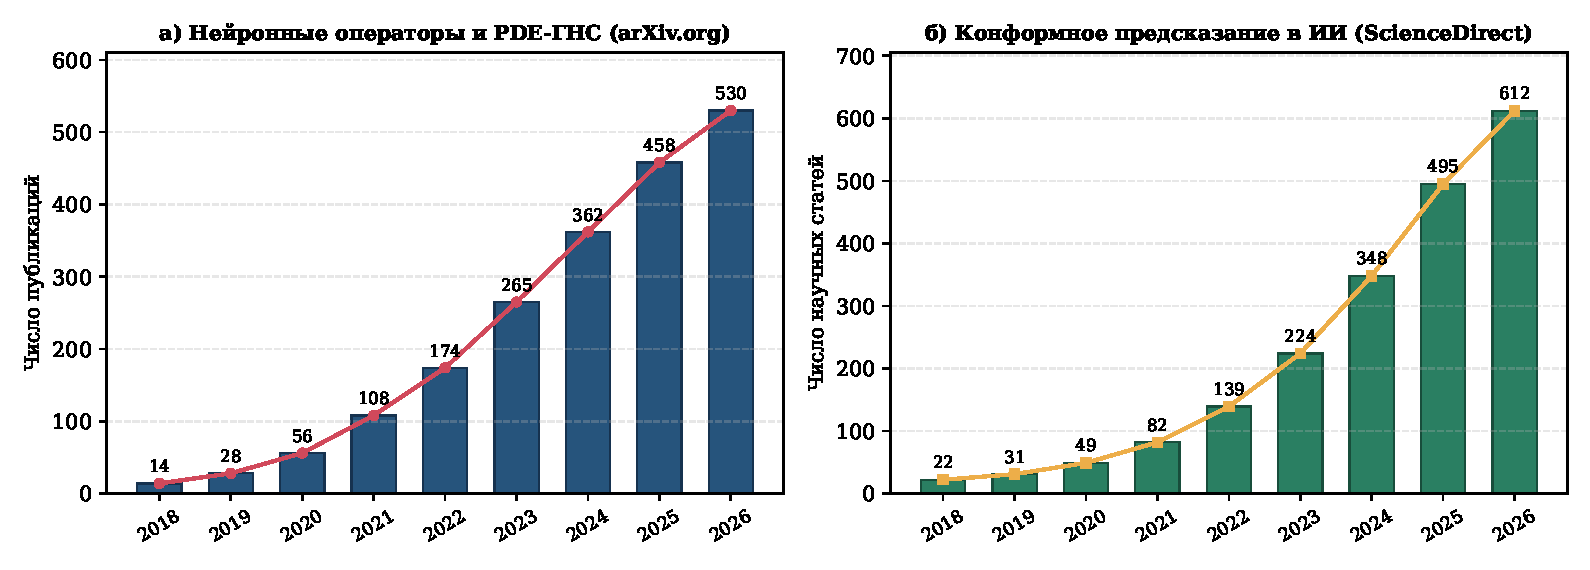
\includegraphics[width=0.98\textwidth]{figures/fig1_pub_dynamics.pdf}
    \caption{Динамика числа научных публикаций за 2018--2026~гг.: а)~по нейронным операторам и графовым УЧП в базе \texttt{arXiv.org}; б)~по конформному предсказанию в ИИ и анализе изображений в базе \texttt{ScienceDirect}}
    \label{fig:pub_dynamics}
\end{figure}

Анализ степени разработанности темы показывает, что спектральные теории переносимости ГНС~[\ref{itm:levie}] опираются на самосопряжённость оператора Лапласа и неприменимы к направленному конвективному сносу, а предельные модели на плотных графонах~[\ref{itm:medvedev},~\ref{itm:yan}] порождают экспоненциально растущие по времени оценки погрешности $\exp(CT)$ и не описывают разреженные планарные сетки. В свою очередь, эмпирические нейронные операторы~[\ref{itm:calvello},~\ref{itm:gfunk}] не снабжают прогнозируемые морфометрические показатели статистически достоверными границами ошибки без запуска эталонного решателя высокого разрешения. Тем самым в современной инженерии научных информационных систем сформировался разрыв между высокой скоростью обучения графовых суррогатов на грубых данных и требованиями метрологической надёжности при их переносе на целевые сетки диагностики.

Целью реферата является систематизация современных информационных технологий моделирования процессов переноса на графах и разработка программно-алгоритмического комплекса \texttt{CDQuad}, обеспечивающего перенос без дообучения адаптивных конвекционно-диффузионных моделей между сетками разного разрешения со статистической сертификацией ошибки морфометрических измерений на открытом стеке языка Python (\texttt{NumPy}, \texttt{SciPy}~[\ref{itm:scipy}], \texttt{scikit-image}~[\ref{itm:skimage}]).

Методологическую основу и методы исследования составляют системный и сравнительный анализ научно-технической литературы и программных платформ, методы вариационного исчисления, кусочно-линейных конечных элементов и барицентрических конечных объёмов на триангуляциях Делоне, алгоритмы разреженной вычислительной линейной алгебры в форматах \texttt{CSR/CSC}, аппарат непараметрического раздельного конформного предсказания (\emph{split conformal prediction})~[\ref{itm:vovk},~\ref{itm:angelopoulos}] и воспроизводимый вычислительный эксперимент на синтетических и реальных биомедицинских изображениях.

\newpage

\chapter*{\large ОБЩАЯ ХАРАКТЕРИСТИКА РАБОТЫ}
\addcontentsline{toc}{chapter}{ОБЩАЯ ХАРАКТЕРИСТИКА РАБОТЫ}

\textbf{Ключевые слова:} ИНФОРМАЦИОННЫЕ ТЕХНОЛОГИИ АНАЛИЗА ДАННЫХ НА ГРАФАХ, ГРАФОВЫЕ ДИФФЕРЕНЦИАЛЬНЫЕ УРАВНЕНИЯ, КОНВЕКЦИЯ-ДИФФУЗИЯ, ПЕРЕНОСИМОСТЬ МЕЖДУ РАЗРЕШЕНИЯМИ, НЕЙРОННЫЕ ОПЕРАТОРЫ, ЧИСЛО ПЕКЛЕ, ДВОЙСТВЕННЫЙ СЛОВАРНЫЙ ДЕФЕКТ, КОНФОРМНОЕ ПРЕДСКАЗАНИЕ, МОРФОМЕТРИЯ ИЗОБРАЖЕНИЙ, ОТКРЫТОЕ ПРОГРАММНОЕ ОБЕСПЕЧЕНИЕ.

\textbf{Связь работы с научными программами (проектами), темами.} Тема реферата и магистерской диссертации соответствует приоритетному направлению «1.~Цифровые технологии и искусственный интеллект» Указа Президента Республики Беларусь от 1~апреля 2025~г. №~135 «О приоритетных направлениях научной, научно-технической и инновационной деятельности на 2026--2030~годы»~[\ref{itm:ukaz135}], положениям Государственной программы «Цифровое развитие Беларуси»~[\ref{itm:gosprog}] в части создания импортонезависимых алгоритмических и программных средств анализа данных и биомедицинских изображений, а также выполняется в рамках темы НИР кафедры теории вероятностей и математической статистики ФПМИ БГУ «Математические и компьютерные методы анализа данных на графах» (распоряжение по ФПМИ БГУ от 11.09.2026 №~47).

\textbf{Цель и задачи исследования.} Цель работы~-- обоснование, алгоритмизация и программная реализация континуально-согласованного класса адаптивных конвекционно-диффузионных графовых операторов \texttt{CDQuad} и процедуры статистической сертификации ошибки переноса для устойчивой морфометрии динамических структур на изображениях переменного разрешения. Задачи исследования:
\begin{enumerate}
    \item выполнить аналитический обзор литературы 2020--2026~гг. и сравнительный аудит программных библиотек научного машинного обучения на графах;
    \item установить асимптотический механизм вырождения комбинаторных конвекционно-диффузионных ГНС при измельчении шага сетки;
    \item разработать модульный программный комплекс \texttt{CDQuad} на базе разреженных матричных структур \texttt{CSR/CSC} библиотеки \texttt{SciPy};
    \item предложить быстровычислимый эллиптический двойственный дефект сетки в норме $H_G^{-1}$ и построить процедуру раздельной конформной калибровки ошибки без эталонного решателя;
    \item верифицировать технологию на синтетических сериях и реальной цейтраферной флуоресцентной микроскопии с локализацией границ применимости.
\end{enumerate}

\textbf{Объект и предмет исследования.} Объект исследования~-- информационные технологии, математические модели и программные комплексы пространственно-временного анализа данных на геометрических графах и расчётных сетках. Предмет исследования~-- квадратурно-согласованные конвекционно-диффузионные графовые операторы, алгоритмы непараметрической конформной сертификации ошибки дискретизации и методы вычислительной морфометрии динамических изображений.

\textbf{Научная новизна и практическая значимость.} Показано, что сочетание кусочно-линейной конечно-элементной жёсткости анизотропного тензора диффузии $K(x)$ с консервативными противопоточными потоками на барицентрических дуальных ячейках Дональда и нелокальным вентилем фиксированного физического радиуса $r_0>0$ выводит бездивергентный перенос из показателя экспоненты Гронуолла, обеспечивая линейный масштаб ошибки по числу Пекле и равномерную устойчивость на $t\in[0,\infty)$. Для сертификации смены пространственной сетки без эталонного решателя введён эллиптический двойственный словарный дефект в $H_G^{-1}$, повышающий корреляцию с истинной ошибкой с $0{,}5590$ до $0{,}9803$ и сокращающий ширину конформного интервала на $27{,}9\text{--}36{,}5\,\%$. Практическая значимость состоит в создании открытого кроссплатформенного пакета на языке Python, снижающего ошибку прогноза поля при $8{,}4$-кратном росте числа узлов в $2{,}28$~раза и уменьшающего межмасштабный дрейф на реальной живой микроскопии в $4{,}1\text{--}4{,}4$~раза.

\textbf{Апробация работы и опубликованность результатов.} Основные положения докладывались на XII~Международной научно-практической конференции «BIG DATA and Advanced Analytics» (Минск, БГУИР, 23~апреля 2026~г.), 83-й научной конференции студентов и аспирантов БГУ (Минск, 2026) и научных семинарах ФПМИ БГУ. Опубликованы 4~научные работы соискателя~[\ref{itm:a1}--\ref{itm:a2}], включая статью в журнале «Вестник БГУ. Серия~1»~[\ref{itm:a1}] и статью в сборнике международной конференции БГУИР~[\ref{itm:a_grade}]. Подготовлены презентация из 15~слайдов (Приложение~А) и персональный научно-образовательный веб-ресурс (Приложение~Б).

\textbf{Структура и объём реферата.} Реферат включает оглавление, введение, общую характеристику работы, три главы основной части, заключение, список использованных источников (31~наименование: 27~источников библиографического списка и 4~публикации соискателя) и два приложения. Работа содержит 7~рисунков (включая векторную архитектурную схему) и 4~таблицы.

\newpage
